\documentclass[conference]{IEEEtran}
\IEEEoverridecommandlockouts
\usepackage{cite}
\usepackage{amsmath,amssymb,amsfonts}
\usepackage{graphicx}
\usepackage{textcomp}
\usepackage{xcolor}
\usepackage{url}
\def\BibTeX{{\rm B\kern-.05em{\sc i\kern-.025em b}\kern-.08em T\kern-.1667em\lower.7ex\hbox{E}\kern-.125em X}}

\begin{document}

\title{Real-Time Speech Noise Reduction Using Digital Filters: A Causal versus Offline Comparison of Butterworth and Notch Filters}

\author{\IEEEauthorblockN{Author Name}
\IEEEauthorblockA{Department of Electronics and Communication Engineering\\
Institution Name, City, Country\\
email@example.com}}

\maketitle

\begin{abstract}
Digital filters remain the lowest-cost route to suppressing narrowband and band-limited noise in speech, yet reported gains are often measured with offline zero-phase filtering that cannot run in real time. This paper compares four filter families, Butterworth low-pass (LPF), high-pass (HPF), band-pass (BPF) and IIR notch filters, on real speech corrupted with synthetic white, mains-hum, rumble and hiss noise. Each filter is evaluated both as a true causal, frame-by-frame streaming filter and as an offline forward--backward (zero-phase) filter, using SNR, SNR improvement ($\Delta$SNR) and mean squared error (MSE). Over 6 clips, 7 noise conditions and 10 noise realisations per cell, the causal LPF gives $+2.89$~dB $\Delta$SNR for 5~dB white noise and $+11.46$~dB for high-frequency hiss, while a three-harmonic notch bank gives $+11.49$~dB against 50~Hz hum (causal) and $+16.70$~dB (zero-phase). Causal HPF and BPF show negative waveform $\Delta$SNR despite removing noise power, because their group delay of about 6~ms near 100~Hz distorts the waveform; a phase-insensitive output-referred metric and a zero-phase evaluation expose this effect. Streaming output is bit-identical to batch causal filtering. All code, data and results are provided.
\end{abstract}

\begin{IEEEkeywords}
speech enhancement, noise reduction, Butterworth filter, notch filter, real-time processing, causal filtering, zero-phase filtering
\end{IEEEkeywords}

\section{Introduction}
Background noise degrades the quality and intelligibility of speech in telephony, hearing aids and voice interfaces. Modern deep-learning enhancers have advanced rapidly \cite{wang2018supervised,das2021fundamentals,michelsanti2021overview}, but classical digital filters remain attractive on resource-constrained hardware because they need no training data, have a few multiply--accumulates per sample, and have analytically known latency. Filters are also the right tool when the interference has a known spectral location, such as mains hum at 50 or 60~Hz, low-frequency rumble, or out-of-band hiss.

A practical issue is often overlooked: many filter evaluations use zero-phase (forward--backward) filtering, which needs future samples and is therefore not causal. A real-time system must use a causal filter, whose phase response introduces frequency-dependent delay. This paper therefore asks two questions: (i)~which of LPF, HPF, BPF and notch filters best removes which type of noise, and (ii)~how much of the benefit survives when the filter is run causally in a frame-by-frame streaming implementation?

The contributions are: a reproducible comparison of five Butterworth/notch filter configurations under seven noise conditions; an explicit causal-versus-offline analysis with delay compensation; a streaming implementation verified to equal batch causal filtering; and a complete MATLAB/Octave and Python code base with the speech data used.

\section{Related Work}
Supervised deep-learning methods now dominate single-channel speech enhancement; Wang and Chen survey the field \cite{wang2018supervised}, and Das \textit{et al.} and Michelsanti \textit{et al.} give broader and audio-visual overviews \cite{das2021fundamentals,michelsanti2021overview}. Early neural approaches include WaveNet-style waveform denoising \cite{rethage2018wavenet}. Recent surveys cover generative adversarial approaches \cite{ramonaite2026gan} and diffusion models for audio restoration \cite{lemercier2024diffusion}.

Real-time operation has been a focus of recent work. Valin combined DSP and deep learning for full-band enhancement \cite{valin2018hybrid}. The Interspeech 2020 Deep Noise Suppression Challenge provided datasets and a subjective testing framework for real-time single-channel enhancement and observed that common objective metrics correlate poorly with subjective tests \cite{reddy2020dns}. Entries and later models include a causal waveform-domain model that runs in real time on a laptop CPU \cite{defossez2020real}, the complex-valued DCCRN \cite{hu2020dccrn}, the small DTLN \cite{westhausen2020dtln}, FullSubNet \cite{hao2021fullsubnet}, and the low-complexity DeepFilterNet \cite{schroeter2022deepfilternet} with its successors, which report real-time factors of 0.04 on a notebook CPU for embedded-oriented operation \cite{schroeter2022dfn2} and 0.19 on a single thread for a perceptually motivated version \cite{schroeter2023dfn3}. These systems target broadband, non-stationary noise and need training data and considerably more computation than a biquad cascade. The present paper addresses the complementary, well-defined case in which the noise has a known spectral signature and a classical filter suffices, and it quantifies what causality costs.

\section{Methodology}
\subsection{Signal model and metrics}
A clean speech signal $s[n]$ is corrupted by additive noise $n[n]$:
\begin{equation}
x[n]=s[n]+n[n],\qquad \mathrm{SNR_{in}}=10\log_{10}\frac{\sum_n s^2[n]}{\sum_n n^2[n]}.
\label{eq:model}
\end{equation}
The noise is scaled so that $\mathrm{SNR_{in}}$ equals its target exactly for every clip. A filter $H$ produces $\hat{s}=H\{x\}$, and the waveform metrics against the clean reference are
\begin{align}
\mathrm{SNR_{out}}&=10\log_{10}\frac{\sum_n s^2[n]}{\sum_n (s[n]-\hat{s}[n])^2},\label{eq:snrout}\\
\Delta\mathrm{SNR}&=\mathrm{SNR_{out}}-\mathrm{SNR_{in}},\label{eq:dsnr}\\
\mathrm{MSE}&=\frac{1}{N}\sum_{n=0}^{N-1}\big(s[n]-\hat{s}[n]\big)^2.\label{eq:mse}
\end{align}
Because \eqref{eq:snrout} compares waveforms, it penalises both residual noise and any speech distortion or delay introduced by the filter. Since all filters here are linear, $\hat{s}=H\{s\}+H\{n\}$, which allows a complementary output-referred SNR that is independent of filter delay and phase:
\begin{equation}
\mathrm{SNR_{oref}}=10\log_{10}\frac{\sum_n (H\{s\}[n])^2}{\sum_n (H\{n\}[n])^2}.
\label{eq:oref}
\end{equation}
A third, phase-insensitive metric applies \eqref{eq:snrout} to STFT magnitudes (512-point Hann window, 50\% overlap). All clips are scaled to RMS $0.1$, so MSE values are comparable across clips and $\mathrm{MSE_{in}}=0.01\cdot10^{-\mathrm{SNR_{in}}/10}$.

\subsection{Filters}
The Butterworth magnitude response of order $N$ and cut-off $f_c$ is
\begin{equation}
|H_{\mathrm{LP}}(f)|^2=\frac{1}{1+(f/f_c)^{2N}},\qquad |H_{\mathrm{HP}}(f)|^2=\frac{1}{1+(f_c/f)^{2N}}.
\label{eq:butter}
\end{equation}
Digital filters are obtained by the bilinear transform with pre-warping, and are implemented as cascaded second-order sections (biquads) in transposed direct form~II,
\begin{equation}
y[n]=b_0x[n]+b_1x[n-1]+b_2x[n-2]-a_1y[n-1]-a_2y[n-2],
\label{eq:biquad}
\end{equation}
which is numerically robust for the 100~Hz corner at $f_s=16$~kHz. The notch filter at $f_0$ with quality factor $Q$ is
\begin{equation}
H_{\mathrm{N}}(z)=g\,\frac{1-2\cos\omega_0 z^{-1}+z^{-2}}{1-2g\cos\omega_0 z^{-1}+(2g-1)z^{-2}},
\label{eq:notch}
\end{equation}
with $\omega_0=2\pi f_0/f_s$, $\beta=\tan(\omega_0/(2Q))$ and $g=1/(1+\beta)$. Table~\ref{tab:filters} lists the five configurations.

\begin{table}[!t]
\caption{Filter configurations ($f_s=16$~kHz).}
\label{tab:filters}
\centering\footnotesize
\begin{tabular}{lll}
\hline
Name & Design & Parameters \\ \hline
LPF & Butterworth low-pass & $N=4$, $f_c=3400$~Hz \\
HPF & Butterworth high-pass & $N=4$, $f_c=100$~Hz \\
BPF & Butterworth band-pass & $N=4$ (8th order), 100--3400~Hz \\
Notch & Single IIR notch & $f_0=50$~Hz, $Q=30$ \\
Notch-H & Notch bank & $f_0\in\{50,100,150\}$~Hz, $Q=30$ \\ \hline
\end{tabular}
\end{table}

\subsection{Causal (real-time) versus offline filtering}
A causal filter computes $y[n]$ from $x[m]$, $m\le n$, so it can run sample-by-sample or frame-by-frame with state carried across frames, and its only inherent delay is its group delay
\begin{equation}
\tau_g(\omega)=-\frac{d\,\angle H(e^{j\omega})}{d\omega}.
\label{eq:gd}
\end{equation}
Butterworth filters are minimum-phase-like but not linear-phase, so $\tau_g$ varies with frequency (Fig.~\ref{fig:resp}c). The total algorithmic latency of a streaming implementation is the frame-buffering time plus $\tau_g$.

Offline zero-phase filtering runs the filter forward, reverses the output, runs it again and reverses it back:
\begin{equation}
y_z=\mathcal{R}\{H\{\mathcal{R}\{H\{x\}\}\}\},\qquad |H_z(f)|=|H(f)|^2,\quad \angle H_z=0,
\label{eq:zp}
\end{equation}
where $\mathcal{R}$ reverses the sequence. This requires the whole signal (future samples), so it is \emph{not} real-time. It doubles the attenuation in dB and moves the $-3$~dB corner to $-6$~dB (Fig.~\ref{fig:resp}b).

For the causal outputs two evaluations are reported. \emph{Raw} compares $\hat{s}[n]$ with $s[n]$ directly. \emph{Delay-compensated} advances $\hat{s}$ by the integer lag $\tau\in[0,160]$ samples that maximises the cross-correlation between $s$ and $H\{s\}$, a bulk-delay correction that is available only offline but shows how much error is due to a pure delay. A single integer lag cannot remove frequency-dependent delay, which is the central finding below.

\subsection{Experimental setup}
\textbf{Speech.} Six real utterances (19.4~s in total) from the CMU Arctic corpus (two speakers, 16~kHz, mono) were taken from the pyroomacoustics repository example data. DC was removed and each clip scaled to RMS $0.1$.\\
\textbf{Noise.} Seven conditions were synthesised with seeded generators: white Gaussian noise (WGN) at 0, 5 and 10~dB; mains hum with components at 50, 100 and 150~Hz (relative amplitudes $1$, $0.5$, $0.25$, random phases) at 5~dB; rumble (20--80~Hz band-limited noise) at 5~dB; hiss (5--7.9~kHz band-limited noise) at 5~dB; and hum plus WGN of equal power at 5~dB total.\\
\textbf{Trials.} Each condition--filter--mode cell uses 6 clips $\times$ 10 noise seeds $=60$ trials; tables give mean $\pm$ standard deviation.\\
\textbf{Streaming.} The causal filters were also run frame-by-frame (5, 10, 20 and 32~ms frames) with state carried between frames and compared with batch causal output; per-frame processing time was measured.\\
\textbf{Software.} The main results were produced with Python (NumPy 2.4.4, SciPy 1.17.1). The MATLAB implementation was executed in GNU Octave 8.4.0 (not in MATLAB) and agreed with the Python results (Section~\ref{sec:valid}). Fig.~\ref{fig:block} shows the system and Fig.~\ref{fig:flow} the experimental procedure.

\begin{figure*}[!t]
\centering
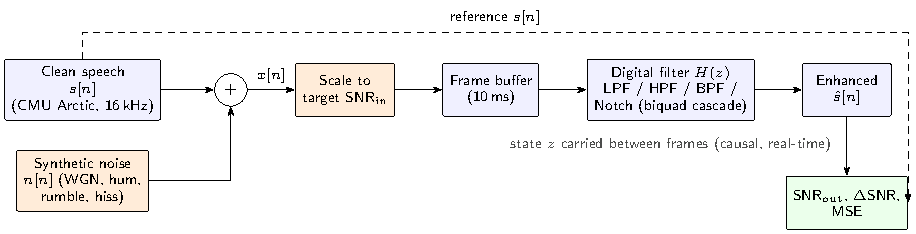
\includegraphics[width=0.95\textwidth]{figures/fig_block_diagram.pdf}
\caption{System block diagram of the evaluation chain with frame-based causal filtering.}
\label{fig:block}
\end{figure*}

\begin{figure}[!t]
\centering
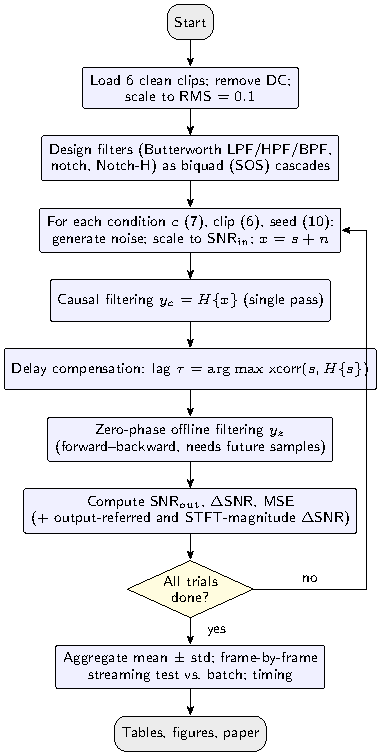
\includegraphics[height=0.40\textheight]{figures/fig_flowchart.pdf}
\caption{Methodology flowchart.}
\label{fig:flow}
\end{figure}

\begin{figure*}[!t]
\centering
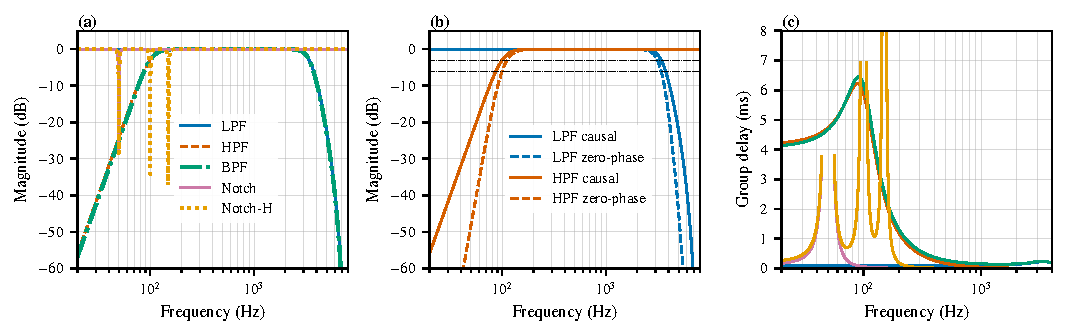
\includegraphics[width=\textwidth]{figures/fig_filter_response.pdf}
\caption{Filter responses. (a)~Magnitude responses of the five filters. (b)~Causal versus zero-phase magnitude of LPF and HPF (dotted lines: $-3$ and $-6$~dB). (c)~Group delay; spikes near notch centres are where group delay is undefined.}
\label{fig:resp}
\end{figure*}

\section{Results}
\subsection{Waveforms and spectra}
Fig.~\ref{fig:wave} shows one utterance in 5~dB white noise and the causal LPF and BPF outputs. Fig.~\ref{fig:spec} (top left) shows that the white noise floor dominates the speech spectrum above about 3~kHz, which the LPF and BPF remove; Fig.~\ref{fig:spec} (top right) shows that the 50~Hz hum peak is reduced by the single notch and further, together with the 100 and 150~Hz harmonics, by the notch bank. The spectrograms in the lower half of Fig.~\ref{fig:spec} show the same behaviour in the time--frequency plane.

\begin{figure}[!t]
\centering
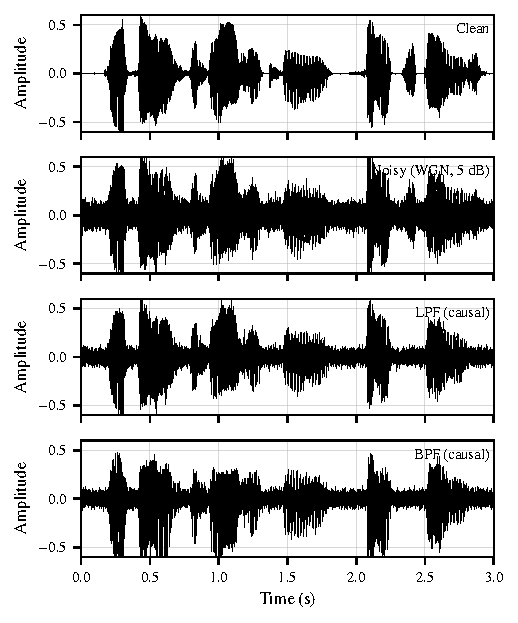
\includegraphics[width=\columnwidth]{figures/fig_waveforms.pdf}
\caption{Clean, noisy (5~dB WGN) and causal LPF/BPF-filtered waveforms (delay-compensated).}
\label{fig:wave}
\end{figure}

\begin{figure*}[!t]
\centering
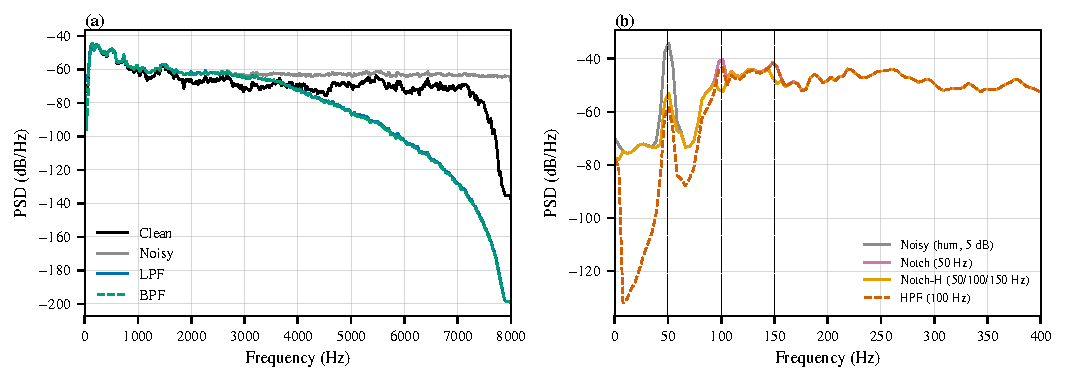
\includegraphics[width=0.9\textwidth]{figures/fig_spectra.pdf}\\[4pt]
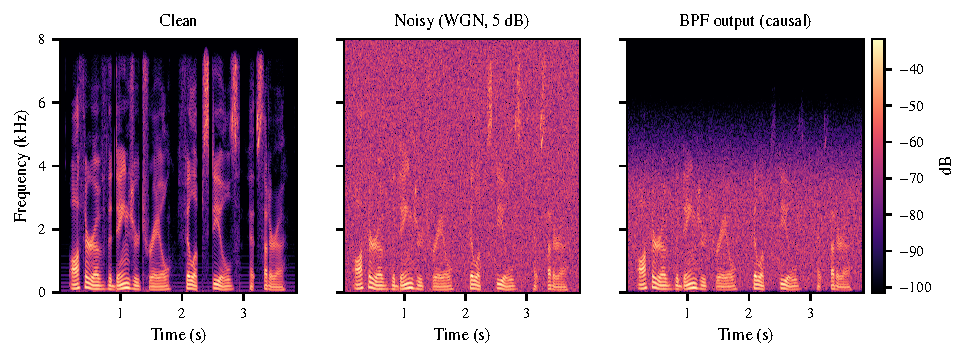
\includegraphics[width=0.9\textwidth]{figures/fig_spectrograms.pdf}
\caption{Frequency-domain views. Top: Welch power spectral densities, (a)~5~dB WGN, full band, and (b)~5~dB hum, 0--400~Hz (dotted lines at 50, 100, 150~Hz). Bottom: spectrograms of the clean signal, the 5~dB WGN mixture and the causal BPF output.}
\label{fig:spec}
\end{figure*}

\subsection{Waveform SNR improvement and MSE}
Tables~\ref{tab:dsnr_causal} and~\ref{tab:mse_causal} give the real-time (causal) results and Table~\ref{tab:dsnr_zp} the offline zero-phase $\Delta$SNR; Fig.~\ref{fig:dsnr} summarises the causal case, and the zero-phase MSE is shown in the lower half of Fig.~\ref{fig:cvz} (all values are in \texttt{results/metrics\_summary.csv}).

\begin{table*}[!t]
\caption{Waveform $\Delta$SNR (dB), real-time causal filtering with integer delay compensation (mean $\pm$ std over 60 trials; best per row in bold).}
\label{tab:dsnr_causal}
\centering\footnotesize
\begin{tabular}{lccccc}
\hline
Condition & LPF & HPF & BPF & Notch & Notch-H \\ \hline
WGN 0 dB & \textbf{3.41 $\pm$ 0.23} & $-$2.74 $\pm$ 0.43 & $-$1.04 $\pm$ 0.73 & 0.00 $\pm$ 0.00 & $-$0.06 $\pm$ 0.06 \\
WGN 5 dB & \textbf{2.89 $\pm$ 0.61} & $-$5.79 $\pm$ 0.69 & $-$4.93 $\pm$ 0.95 & 0.00 $\pm$ 0.00 & $-$0.21 $\pm$ 0.19 \\
WGN 10 dB & \textbf{1.62 $\pm$ 1.33} & $-$9.92 $\pm$ 0.84 & $-$9.50 $\pm$ 1.04 & 0.00 $\pm$ 0.00 & $-$0.63 $\pm$ 0.53 \\
Hum 5 dB & $-$0.38 $\pm$ 0.30 & $-$4.67 $\pm$ 0.89 & $-$4.52 $\pm$ 1.03 & 5.80 $\pm$ 0.16 & \textbf{11.49 $\pm$ 2.36} \\
Rumble 5 dB & $-$0.38 $\pm$ 0.30 & $-$4.51 $\pm$ 0.92 & $-$4.35 $\pm$ 1.08 & \textbf{0.19 $\pm$ 0.05} & $-$0.01 $\pm$ 0.21 \\
Hiss 5 dB & \textbf{11.46 $\pm$ 3.34} & $-$5.80 $\pm$ 0.68 & $-$4.29 $\pm$ 1.09 & 0.00 $\pm$ 0.00 & $-$0.22 $\pm$ 0.19 \\
Hum+WGN 5 dB & 0.95 $\pm$ 0.40 & $-$5.26 $\pm$ 0.77 & $-$4.72 $\pm$ 0.98 & 2.00 $\pm$ 0.04 & \textbf{2.48 $\pm$ 0.32} \\
\hline
\end{tabular}

\end{table*}
\begin{table*}[!t]
\caption{MSE against the clean reference ($\times10^{-3}$, clips normalised to RMS 0.1), causal filtering with delay compensation (mean $\pm$ std; lowest per row in bold).}
\label{tab:mse_causal}
\centering\footnotesize
\begin{tabular}{lcccccc}
\hline
Condition & Unfilt. & LPF & HPF & BPF & Notch & Notch-H \\ \hline
WGN 0 dB & 10.00 & \textbf{4.56 $\pm$ 0.25} & 18.87 $\pm$ 1.86 & 12.89 $\pm$ 2.08 & 10.00 $\pm$ 0.00 & 10.15 $\pm$ 0.15 \\
WGN 5 dB & 3.16 & \textbf{1.64 $\pm$ 0.24} & 12.13 $\pm$ 1.87 & 10.06 $\pm$ 2.09 & 3.16 $\pm$ 0.00 & 3.32 $\pm$ 0.14 \\
WGN 10 dB & 1.00 & \textbf{0.72 $\pm$ 0.24} & 9.99 $\pm$ 1.86 & 9.16 $\pm$ 2.08 & 1.00 $\pm$ 0.00 & 1.16 $\pm$ 0.14 \\
Hum 5 dB & 3.16 & 3.46 $\pm$ 0.24 & 9.45 $\pm$ 1.86 & 9.19 $\pm$ 2.08 & 0.83 $\pm$ 0.03 & \textbf{0.26 $\pm$ 0.12} \\
Rumble 5 dB & 3.16 & 3.46 $\pm$ 0.24 & 9.14 $\pm$ 1.86 & 8.87 $\pm$ 2.08 & \textbf{3.03 $\pm$ 0.03} & 3.17 $\pm$ 0.15 \\
Hiss 5 dB & 3.16 & \textbf{0.30 $\pm$ 0.24} & 12.17 $\pm$ 1.86 & 8.75 $\pm$ 2.08 & 3.16 $\pm$ 0.00 & 3.33 $\pm$ 0.14 \\
Hum+WGN 5 dB & 3.16 & 2.55 $\pm$ 0.24 & 10.77 $\pm$ 1.85 & 9.60 $\pm$ 2.06 & 2.00 $\pm$ 0.02 & \textbf{1.79 $\pm$ 0.13} \\
\hline
\end{tabular}

\end{table*}
\begin{table*}[!t]
\caption{Waveform $\Delta$SNR (dB), offline zero-phase (forward--backward) filtering (mean $\pm$ std over 60 trials; best per row in bold).}
\label{tab:dsnr_zp}
\centering\footnotesize
\begin{tabular}{lccccc}
\hline
Condition & LPF & HPF & BPF & Notch & Notch-H \\ \hline
WGN 0 dB & 3.81 $\pm$ 0.27 & 0.02 $\pm$ 0.03 & \textbf{3.84 $\pm$ 0.34} & 0.00 $\pm$ 0.00 & $-$0.02 $\pm$ 0.04 \\
WGN 5 dB & \textbf{3.28 $\pm$ 0.72} & $-$0.06 $\pm$ 0.11 & 3.15 $\pm$ 0.87 & 0.00 $\pm$ 0.00 & $-$0.09 $\pm$ 0.11 \\
WGN 10 dB & \textbf{2.04 $\pm$ 1.56} & $-$0.32 $\pm$ 0.32 & 1.64 $\pm$ 1.83 & 0.00 $\pm$ 0.00 & $-$0.31 $\pm$ 0.34 \\
Hum 5 dB & $-$0.36 $\pm$ 0.32 & 9.25 $\pm$ 0.94 & 7.27 $\pm$ 2.09 & 6.12 $\pm$ 0.04 & \textbf{16.70 $\pm$ 4.24} \\
Rumble 5 dB & $-$0.36 $\pm$ 0.32 & \textbf{14.88 $\pm$ 3.20} & 10.48 $\pm$ 3.88 & 0.28 $\pm$ 0.06 & 0.22 $\pm$ 0.15 \\
Hiss 5 dB & \textbf{12.51 $\pm$ 4.27} & $-$0.12 $\pm$ 0.11 & 11.38 $\pm$ 4.59 & 0.00 $\pm$ 0.00 & $-$0.11 $\pm$ 0.11 \\
Hum+WGN 5 dB & 1.09 $\pm$ 0.44 & 2.45 $\pm$ 0.20 & \textbf{4.70 $\pm$ 1.23} & 2.06 $\pm$ 0.02 & 2.79 $\pm$ 0.21 \\
\hline
\end{tabular}

\end{table*}

\begin{figure*}[!t]
\centering
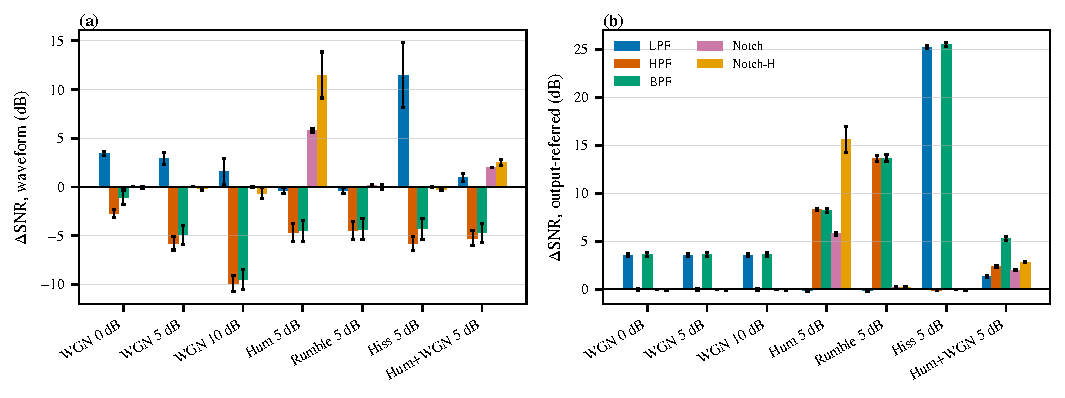
\includegraphics[width=\textwidth]{figures/fig_dsnr_causal.pdf}
\caption{Causal (delay-compensated) $\Delta$SNR per condition: (a)~waveform-referenced, (b)~output-referred. Error bars: one standard deviation over 60 trials.}
\label{fig:dsnr}
\end{figure*}

\subsection{Causal versus offline filtering}
Fig.~\ref{fig:cvz} compares raw causal, delay-compensated causal and zero-phase results for the BPF and LPF. Delay compensation matters for the LPF (e.g.\ $-0.73$~dB raw versus $+2.89$~dB compensated for 5~dB WGN) because the LPF delay is nearly constant ($\approx0.1$~ms) and a 2-sample shift removes most of it. It does not rescue the BPF and HPF, whose delay varies from about 6~ms at 100~Hz to under 0.3~ms above 500~Hz.

\begin{figure*}[!t]
\centering
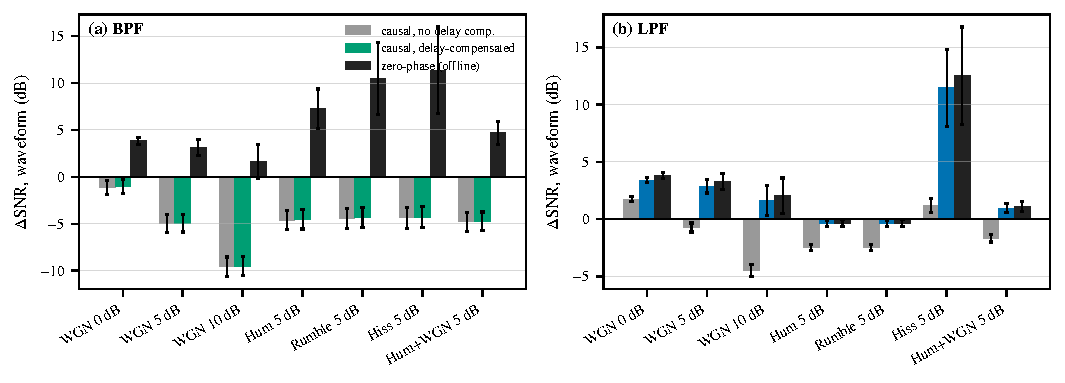
\includegraphics[width=0.9\textwidth]{figures/fig_causal_vs_zerophase.pdf}\\[4pt]
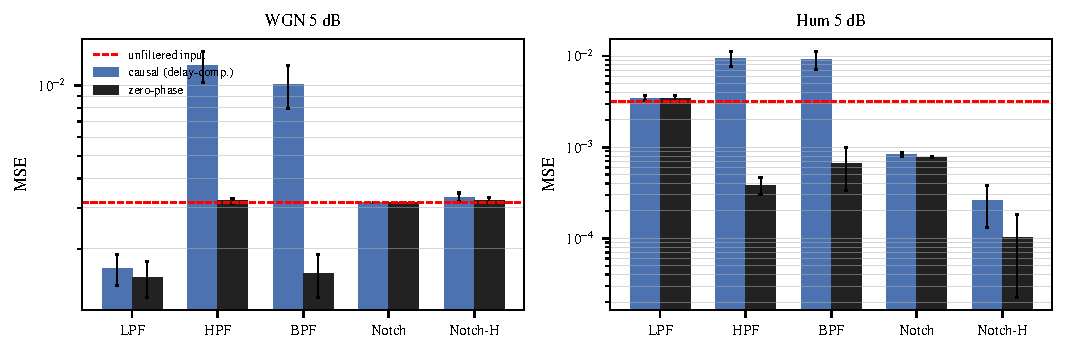
\includegraphics[width=0.9\textwidth]{figures/fig_mse.pdf}
\caption{Top: waveform $\Delta$SNR for raw causal, delay-compensated causal and offline zero-phase filtering, (a)~BPF and (b)~LPF. Bottom: MSE (log scale) for 5~dB WGN and 5~dB hum, delay-compensated causal versus zero-phase; the dashed line is the unfiltered input.}
\label{fig:cvz}
\end{figure*}

\subsection{Delay- and phase-independent metrics}
Table~\ref{tab:dsnr_oref} reports the output-referred $\Delta$SNR of \eqref{eq:oref}. For white noise, the LPF and BPF give 3.6~dB at every input SNR, close to the ideal $10\log_{10}(8000/3400)=3.72$~dB expected from removing the noise above 3.4~kHz from a flat spectrum; the HPF and notches remove almost no white-noise power. For narrowband noise the picture is clear: the HPF and BPF give 13.6~dB against rumble, the LPF and BPF 25.2--25.5~dB against hiss, and the notch bank 15.6~dB against hum (21.6~dB zero-phase). The STFT-magnitude $\Delta$SNR (available in \texttt{results/}) shows the same qualitative picture and, unlike the waveform metric, is positive for the causal HPF and BPF against rumble and hum (e.g.\ $+13.0$~dB for HPF against rumble, causal).

\begin{table*}[!t]
\caption{Output-referred $\Delta$SNR (dB), $10\log_{10}(\|Hs\|^2/\|Hn\|^2)-\mathrm{SNR_{in}}$, causal filtering. This metric is independent of filter delay and phase and isolates noise-power removal.}
\label{tab:dsnr_oref}
\centering\footnotesize
\begin{tabular}{lccccc}
\hline
Condition & LPF & HPF & BPF & Notch & Notch-H \\ \hline
WGN 0 dB & 3.56 $\pm$ 0.13 & $-$0.04 $\pm$ 0.08 & \textbf{3.59 $\pm$ 0.20} & 0.00 $\pm$ 0.00 & $-$0.06 $\pm$ 0.07 \\
WGN 5 dB & 3.57 $\pm$ 0.13 & $-$0.04 $\pm$ 0.08 & \textbf{3.60 $\pm$ 0.20} & 0.00 $\pm$ 0.00 & $-$0.06 $\pm$ 0.07 \\
WGN 10 dB & 3.55 $\pm$ 0.13 & $-$0.04 $\pm$ 0.08 & \textbf{3.58 $\pm$ 0.20} & 0.00 $\pm$ 0.00 & $-$0.06 $\pm$ 0.07 \\
Hum 5 dB & $-$0.14 $\pm$ 0.12 & 8.32 $\pm$ 0.08 & 8.18 $\pm$ 0.20 & 5.80 $\pm$ 0.16 & \textbf{15.62 $\pm$ 1.38} \\
Rumble 5 dB & $-$0.14 $\pm$ 0.12 & 13.61 $\pm$ 0.31 & \textbf{13.68 $\pm$ 0.34} & 0.19 $\pm$ 0.05 & 0.15 $\pm$ 0.09 \\
Hiss 5 dB & 25.24 $\pm$ 0.14 & $-$0.10 $\pm$ 0.08 & \textbf{25.50 $\pm$ 0.20} & 0.00 $\pm$ 0.00 & $-$0.07 $\pm$ 0.07 \\
Hum+WGN 5 dB & 1.33 $\pm$ 0.12 & 2.38 $\pm$ 0.09 & \textbf{5.31 $\pm$ 0.20} & 2.00 $\pm$ 0.04 & 2.82 $\pm$ 0.06 \\
\hline
\end{tabular}

\end{table*}



\subsection{Real-time behaviour}
Table~\ref{tab:rt} and Fig.~\ref{fig:rt} give group delay and streaming measurements. Streaming output was identical to batch causal output for every filter and frame length (maximum absolute difference $0$). In the authors' Python sandbox the mean time per 10~ms frame was 0.03--0.04~ms (real-time factor about 0.003); absolute timings depend on hardware and language and are not claims about embedded targets. With a 10~ms frame, the latency of the LPF, notch and notch bank is dominated by buffering, whereas HPF/BPF add about 6~ms of group delay near 100~Hz.

\begin{table*}[!t]
\caption{Real-time characteristics of the causal filters at $f_s=16$ kHz (frame-by-frame streaming, 10~ms frames). Group delay (GD) from the analytic phase response; ``max GD is the maximum over 100--3400~Hz (excluding $\pm10$~Hz around notch centres, where GD is undefined). Timing was measured on the authors' sandbox CPU with SciPy and will differ on other hardware.}
\label{tab:rt}
\centering\footnotesize
\begin{tabular}{lccccccccc}
\hline
Filter & Order & GD@200\,Hz & GD@1\,kHz & max GD & est. lag & mean time & max time & RTF & max$|$stream$-$batch$|$ \\
 & & (ms) & (ms) & (ms) & samples (ms) & (ms/frame) & (ms/frame) & & \\ \hline
LPF & 4 & 0.10 & 0.11 & 0.24 & 2.0 (0.12) & 0.039 & 0.133 & 0.0039 & 0.0e+00 \\
HPF & 4 & 1.19 & 0.04 & 5.85 & 10.3 (0.65) & 0.032 & 0.099 & 0.0032 & 0.0e+00 \\
BPF & 8 & 1.31 & 0.16 & 6.16 & 10.7 (0.67) & 0.035 & 0.125 & 0.0035 & 0.0e+00 \\
Notch & 2 & 0.01 & 0.00 & 0.06 & 0.0 (0.00) & 0.032 & 0.098 & 0.0032 & 0.0e+00 \\
Notch-H & 6 & 0.20 & 0.00 & 3.96 & 0.0 (0.00) & 0.033 & 0.090 & 0.0033 & 0.0e+00 \\
\hline
\end{tabular}
\end{table*}

\begin{figure*}[!t]
\centering
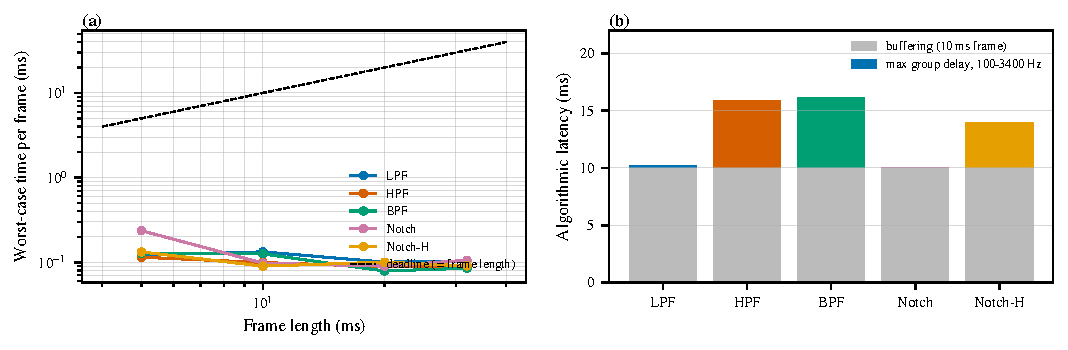
\includegraphics[width=\textwidth]{figures/fig_realtime.pdf}
\caption{(a)~Worst-case processing time per frame versus frame length. (b)~Algorithmic latency: 10~ms buffering plus maximum group delay in 100--3400~Hz (notch centres excluded).}
\label{fig:rt}
\end{figure*}

\subsection{Validation of the MATLAB implementation}
\label{sec:valid}
On a deterministic test (hum with fixed phases, one clip) the Octave-executed MATLAB code and the Python code agreed to within $5\times10^{-7}$~dB in SNR and the $\Delta$SNR variants and to $2.5\times10^{-11}$ in MSE (difference attributable to CSV rounding). On the full randomised experiment, which uses different random-number generators, the mean absolute difference in $\Delta$SNR was 0.004~dB and the maximum 0.11~dB.

\section{Discussion}
\textbf{Matching the filter to the noise.} No single filter is best. The LPF is the best causal choice against white and hiss noise; the notch bank is best against hum; and the HPF is the right tool for rumble, though only the zero-phase version scores well on waveform SNR (Table~\ref{tab:dsnr_zp}). A single 50~Hz notch removes only the fundamental of the hum ($+5.80$~dB) and the three-notch bank doubles the benefit ($+11.49$~dB) because the fundamental carries only about 76\% of the hum power in this model (amplitudes $1$, $0.5$, $0.25$). Against broadband white noise, notches and the HPF do nothing useful (HPF causal $\Delta$SNR $-2.74$ to $-9.92$~dB), and the benefit of LPF/BPF is bounded by the bandwidth argument above, so classical filters are not a substitute for learned enhancers \cite{defossez2020real,hu2020dccrn,schroeter2022deepfilternet} when noise overlaps speech in frequency.

\textbf{Why causality costs waveform SNR.} The causal HPF and BPF have negative waveform $\Delta$SNR in every condition (Table~\ref{tab:dsnr_causal}), including those where the output-referred metric shows large noise removal (Table~\ref{tab:dsnr_oref}). The group delay peaks near the 100~Hz corner (Fig.~\ref{fig:resp}c), exactly where voiced speech has its fundamental and first harmonics, so harmonics are time-shifted relative to higher components. A phase error near $60^\circ$ is enough for the error energy to equal the signal energy, so waveform SNR collapses even though the magnitude spectrum is nearly preserved. Zero-phase filtering removes this term and turns the same BPF into $+3.15$~dB for 5~dB WGN and $+10.48$~dB (waveform) for rumble. The practical consequence is that offline zero-phase numbers overstate what a real-time system will achieve under a waveform metric, while the output-referred and magnitude metrics show that the causal filter still removes the noise. Which metric matters depends on whether perception of phase distortion matters; conventional objective metrics are known to correlate imperfectly with subjective quality \cite{reddy2020dns}, so a listening test is needed to settle this.

\textbf{Practical guidance.} For real-time use, (i)~prefer a low-order LPF or a notch bank when the interference is out-of-band or tonal, (ii)~avoid HPF/BPF corners close to the speech fundamental unless the phase distortion is acceptable, e.g.\ lower the corner or use a lower order, (iii)~budget buffering plus group delay (Fig.~\ref{fig:rt}b), and (iv)~implement filters as biquad cascades with carried state, which here reproduced batch output exactly.

\textbf{Limitations.} The data are six clips from two speakers; the noise is synthetic and stationary; there are no perceptual metrics (PESQ, STOI) or listening tests; cut-off frequencies and orders were fixed a priori rather than optimised per condition; the integer-lag compensation is a coarse proxy; and processing times were measured in a Python sandbox, not on embedded hardware. The $\Delta$SNR of the LPF decreasing from $+3.41$ to $+1.62$~dB as input SNR rises from 0 to 10~dB is consistent with the constant 3.6~dB noise removal being offset by distortion of speech content above 3.4~kHz and by residual phase error, but this attribution was not isolated by a separate experiment.

\section{Conclusion}
Using real speech and seeded synthetic noise, a causal LPF improved waveform SNR by $+2.89$~dB (5~dB WGN) and $+11.46$~dB (hiss), and a three-notch bank by $+11.49$~dB against 50~Hz hum, while a single notch gave $+5.80$~dB. Causal HPF and BPF filters removed noise power (up to 13.6~dB output-referred for rumble) but lost waveform SNR through frequency-dependent group delay of about 6~ms near 100~Hz; offline zero-phase filtering hides this cost. Frame-by-frame streaming reproduced batch causal output exactly with sub-millisecond processing time per 10~ms frame in the test environment. Future work should add perceptual metrics and listening tests, real recorded noise, adaptive notch/cut-off selection and implementation on embedded targets.

\section*{Reproducibility}
Code (MATLAB/Octave and Python), the speech clips, per-trial results (\texttt{metrics\_raw.csv}) and all figures are included in the accompanying archive; see its README.

\bibliographystyle{IEEEtran}
\bibliography{references}

\end{document}
